\PassOptionsToPackage{unicode=true}{hyperref} % options for packages loaded elsewhere
\PassOptionsToPackage{hyphens}{url}
%
\documentclass[]{article}
\usepackage{lmodern}
\usepackage{amssymb,amsmath}
\usepackage{ifxetex,ifluatex}
\usepackage{fixltx2e} % provides \textsubscript
\ifnum 0\ifxetex 1\fi\ifluatex 1\fi=0 % if pdftex
  \usepackage[T1]{fontenc}
  \usepackage[utf8]{inputenc}
  \usepackage{textcomp} % provides euro and other symbols
\else % if luatex or xelatex
  \usepackage{unicode-math}
  \defaultfontfeatures{Ligatures=TeX,Scale=MatchLowercase}
\fi
% use upquote if available, for straight quotes in verbatim environments
\IfFileExists{upquote.sty}{\usepackage{upquote}}{}
% use microtype if available
\IfFileExists{microtype.sty}{%
\usepackage[]{microtype}
\UseMicrotypeSet[protrusion]{basicmath} % disable protrusion for tt fonts
}{}
\IfFileExists{parskip.sty}{%
\usepackage{parskip}
}{% else
\setlength{\parindent}{0pt}
\setlength{\parskip}{6pt plus 2pt minus 1pt}
}
\usepackage{hyperref}
\hypersetup{
            pdftitle={Using Python with R Markdown},
            pdfauthor={Temple Davies},
            pdfborder={0 0 0},
            breaklinks=true}
\urlstyle{same}  % don't use monospace font for urls
\usepackage[margin=1in]{geometry}
\usepackage{color}
\usepackage{fancyvrb}
\newcommand{\VerbBar}{|}
\newcommand{\VERB}{\Verb[commandchars=\\\{\}]}
\DefineVerbatimEnvironment{Highlighting}{Verbatim}{commandchars=\\\{\}}
% Add ',fontsize=\small' for more characters per line
\usepackage{framed}
\definecolor{shadecolor}{RGB}{248,248,248}
\newenvironment{Shaded}{\begin{snugshade}}{\end{snugshade}}
\newcommand{\AlertTok}[1]{\textcolor[rgb]{0.94,0.16,0.16}{#1}}
\newcommand{\AnnotationTok}[1]{\textcolor[rgb]{0.56,0.35,0.01}{\textbf{\textit{#1}}}}
\newcommand{\AttributeTok}[1]{\textcolor[rgb]{0.77,0.63,0.00}{#1}}
\newcommand{\BaseNTok}[1]{\textcolor[rgb]{0.00,0.00,0.81}{#1}}
\newcommand{\BuiltInTok}[1]{#1}
\newcommand{\CharTok}[1]{\textcolor[rgb]{0.31,0.60,0.02}{#1}}
\newcommand{\CommentTok}[1]{\textcolor[rgb]{0.56,0.35,0.01}{\textit{#1}}}
\newcommand{\CommentVarTok}[1]{\textcolor[rgb]{0.56,0.35,0.01}{\textbf{\textit{#1}}}}
\newcommand{\ConstantTok}[1]{\textcolor[rgb]{0.00,0.00,0.00}{#1}}
\newcommand{\ControlFlowTok}[1]{\textcolor[rgb]{0.13,0.29,0.53}{\textbf{#1}}}
\newcommand{\DataTypeTok}[1]{\textcolor[rgb]{0.13,0.29,0.53}{#1}}
\newcommand{\DecValTok}[1]{\textcolor[rgb]{0.00,0.00,0.81}{#1}}
\newcommand{\DocumentationTok}[1]{\textcolor[rgb]{0.56,0.35,0.01}{\textbf{\textit{#1}}}}
\newcommand{\ErrorTok}[1]{\textcolor[rgb]{0.64,0.00,0.00}{\textbf{#1}}}
\newcommand{\ExtensionTok}[1]{#1}
\newcommand{\FloatTok}[1]{\textcolor[rgb]{0.00,0.00,0.81}{#1}}
\newcommand{\FunctionTok}[1]{\textcolor[rgb]{0.00,0.00,0.00}{#1}}
\newcommand{\ImportTok}[1]{#1}
\newcommand{\InformationTok}[1]{\textcolor[rgb]{0.56,0.35,0.01}{\textbf{\textit{#1}}}}
\newcommand{\KeywordTok}[1]{\textcolor[rgb]{0.13,0.29,0.53}{\textbf{#1}}}
\newcommand{\NormalTok}[1]{#1}
\newcommand{\OperatorTok}[1]{\textcolor[rgb]{0.81,0.36,0.00}{\textbf{#1}}}
\newcommand{\OtherTok}[1]{\textcolor[rgb]{0.56,0.35,0.01}{#1}}
\newcommand{\PreprocessorTok}[1]{\textcolor[rgb]{0.56,0.35,0.01}{\textit{#1}}}
\newcommand{\RegionMarkerTok}[1]{#1}
\newcommand{\SpecialCharTok}[1]{\textcolor[rgb]{0.00,0.00,0.00}{#1}}
\newcommand{\SpecialStringTok}[1]{\textcolor[rgb]{0.31,0.60,0.02}{#1}}
\newcommand{\StringTok}[1]{\textcolor[rgb]{0.31,0.60,0.02}{#1}}
\newcommand{\VariableTok}[1]{\textcolor[rgb]{0.00,0.00,0.00}{#1}}
\newcommand{\VerbatimStringTok}[1]{\textcolor[rgb]{0.31,0.60,0.02}{#1}}
\newcommand{\WarningTok}[1]{\textcolor[rgb]{0.56,0.35,0.01}{\textbf{\textit{#1}}}}
\usepackage{graphicx,grffile}
\makeatletter
\def\maxwidth{\ifdim\Gin@nat@width>\linewidth\linewidth\else\Gin@nat@width\fi}
\def\maxheight{\ifdim\Gin@nat@height>\textheight\textheight\else\Gin@nat@height\fi}
\makeatother
% Scale images if necessary, so that they will not overflow the page
% margins by default, and it is still possible to overwrite the defaults
% using explicit options in \includegraphics[width, height, ...]{}
\setkeys{Gin}{width=\maxwidth,height=\maxheight,keepaspectratio}
\setlength{\emergencystretch}{3em}  % prevent overfull lines
\providecommand{\tightlist}{%
  \setlength{\itemsep}{0pt}\setlength{\parskip}{0pt}}
\setcounter{secnumdepth}{0}
% Redefines (sub)paragraphs to behave more like sections
\ifx\paragraph\undefined\else
\let\oldparagraph\paragraph
\renewcommand{\paragraph}[1]{\oldparagraph{#1}\mbox{}}
\fi
\ifx\subparagraph\undefined\else
\let\oldsubparagraph\subparagraph
\renewcommand{\subparagraph}[1]{\oldsubparagraph{#1}\mbox{}}
\fi

% set default figure placement to htbp
\makeatletter
\def\fps@figure{htbp}
\makeatother


\title{Using Python with R Markdown}
\author{Temple Davies}
\date{2019-12-15}

\begin{document}
\maketitle

This post shows how the package \emph{reticulate} can be utilized in an
R Markdown to converse to python. This example uses matrices and their
properties to explore differnt characteristics of python.

First, a randamized matrix is made in a r code block.

\begin{Shaded}
\begin{Highlighting}[]
\KeywordTok{set.seed}\NormalTok{(}\DecValTok{123}\NormalTok{)}
\NormalTok{matrix <-}\StringTok{ }\KeywordTok{matrix}\NormalTok{(}\KeywordTok{round}\NormalTok{(}\DecValTok{13} \OperatorTok{*}\StringTok{ }\KeywordTok{rexp}\NormalTok{(}\DecValTok{200}\NormalTok{)), }\DecValTok{10}\NormalTok{)}
\end{Highlighting}
\end{Shaded}

This matrix variable can be called in a python code block and converted
to an array. Numpy can also imported so it's functions can be used on
the array.

\begin{Shaded}
\begin{Highlighting}[]
\ImportTok{import}\NormalTok{ numpy }\ImportTok{as}\NormalTok{ np}
\NormalTok{array }\OperatorTok{=}\NormalTok{ r.matrix}
\BuiltInTok{print}\NormalTok{(array)}
\end{Highlighting}
\end{Shaded}

\begin{verbatim}
## [[ 11.  13.  11.  28.   5.   1.  13.  21.   7.   0.   6.   2.   3.   3.
##     9.   2.  14.  19.   7.   9.]
##  [  7.   6.  13.   7.  94.   4.   4.  21.   3.  14.   3.  13.  23.   6.
##    21.  20.  14.  17.  57.  21.]
##  [ 17.   4.  19.   3.  11.  14.  20.  33.  58.   4.  15.   4.  23.   5.
##     8.   1.  49.  19.   7.   1.]
##  [  0.   5.  18.  34.   3.   4.   1.  20.  24.  15.   1.  17.  11.  45.
##     1.   7.   0.  28.   6.   5.]
##  [  1.   2.  15.  16.  14.  13.   1.   5.   9.  14.   5.   4.   5.  17.
##     4.  23.   0.  19.   3.  36.]
##  [  4.  11.  21.  10.  29.  25.   1.   3.  19.   1.  12.  21.  43.  14.
##    23.  17.  22.  11.   9.  37.]
##  [  4.  20.  19.   8.  18.   7.   4.   6.  23.   6.   5.   2.   5.   4.
##     3.  17.   7.  35.  13.   0.]
##  [  2.   6.  20.  16.   7.  34.   4.   1.  16.  20.  10.  23.  14.   1.
##    12.   6.   6.  29.  10.   6.]
##  [ 35.   8.   0.   8.  35.  14.  13.   4.  19.   3.   2.   0.  17.  38.
##     6.   0.   1.   7.  14.   9.]
##  [  0.  53.   8.  15.  17.  13.  12.   8.  20.  24.  11.  17.   8.  26.
##    17.   2.   7.   1.   8.  12.]]
\end{verbatim}

\begin{Shaded}
\begin{Highlighting}[]
\NormalTok{mean }\OperatorTok{=}\NormalTok{ np.mean(array)}
\BuiltInTok{print}\NormalTok{(}\StringTok{"Using numpy, it is found that the mean of the array is }\SpecialCharTok\NormalTok{ mean)}
\end{Highlighting}
\end{Shaded}

\begin{verbatim}
## Using numpy, it is found that the mean of the array is 13.06.
\end{verbatim}

\begin{Shaded}
\begin{Highlighting}[]
\NormalTok{std }\OperatorTok{=}\NormalTok{ np.std(array)}
\BuiltInTok{print}\NormalTok{(}\StringTok{"The standard deviation is determined to be }\SpecialCharTok\NormalTok{ std)}
\end{Highlighting}
\end{Shaded}

\begin{verbatim}
## The standard deviation is determined to be 12.57
\end{verbatim}

\begin{Shaded}
\begin{Highlighting}[]
\KeywordTok{median}\NormalTok{(py}\OperatorTok{$}\NormalTok{array)}
\end{Highlighting}
\end{Shaded}

\begin{verbatim}
## [1] 10
\end{verbatim}

The python variable \emph{array} can be called in the r code block to
determine that the median is 10.

Arrays are considered to be 2-D lists in python. Lists have a unique
feature, called \textbf{indexing}, which allows elements in the list to
be accessed. When indexing, the first element is considered ``0'', the
second ``1'', and so on like as follows:

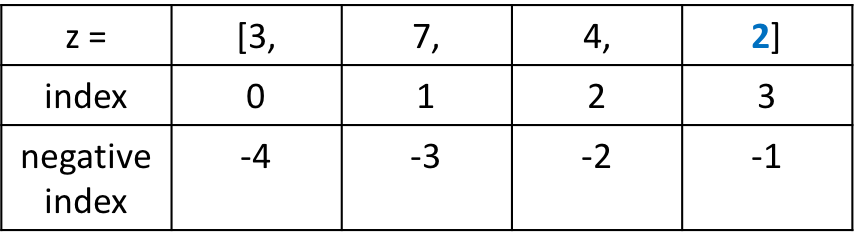
\includegraphics{~/Desktop/website/static/img/index.png}

List slicing uses indexing to access multiple elements in the list. For
a list being cut using the code \emph{my\_list{[}4:7{]}}, the following
occurs:

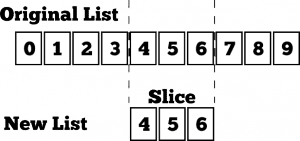
\includegraphics{~/Desktop/website/static/img/slice.png}

Therefore, the array's elemets can be accessed using indexing and
slicing.

\begin{Shaded}
\begin{Highlighting}[]
\NormalTok{array[}\DecValTok{5}\NormalTok{][}\DecValTok{3}\NormalTok{:}\DecValTok{9}\NormalTok{]}
\end{Highlighting}
\end{Shaded}

\begin{verbatim}
## array([ 10.,  29.,  25.,   1.,   3.,  19.])
\end{verbatim}

By using the index operations above on the array, the 6th row from the
array is retrieved. Within that row, the 4th through 9th element are
then returned.

\begin{Shaded}
\begin{Highlighting}[]
\NormalTok{array[}\DecValTok{8}\NormalTok{].}\BuiltInTok{sum}\NormalTok{()}
\end{Highlighting}
\end{Shaded}

\begin{verbatim}
## 233.0
\end{verbatim}

The sum of the 9th row is 233.0.

\end{document}
